\section{Ranking Algorithms}
When a search is done on our search-engine, the method \code{getMachingQueries} in \code{QueryHandler} finds all the websites that matches the query. But of course some of the matching websites are more relevant than others, for the given query. To show the user the most relevant pages at the top, we need a way to rank the websites according to relevance, i.e we need a ranking algorithm. There are many different ways to rank a website, we have chosen to implement the term-frequency algorithm (TF-algorithm), the term-frequency inverse-document-frequency (TFIDF-algorithm), and also our own  term-frequency inverse-corpus-frequency (TFICF-algorithm).    

\subsection{Term Frequency}
Keeping in line with the notation at \cite{wikiTFIDF} the term frequency, TF, is calculated as follows.

\[ TF = \frac{f_{t,d}}{\sum_{i \in d}f_{i,d}} \]

Note that we have choosen the term frequency that is weighted by the total number of words in the document/site. The corresponding Java implementation is shown in listing \ref{lst:tf}.

\begin{lstlisting}[language=Java,
					caption={Implementation of calculating TF rating.},
					label={lst:tf}]
/**
* Rank a single website according to a single word. Ranking algorithm is TF
* 
* @param site a single website that will be ranked.
* @param a single word from the search query.
* @return the rank of the site. Rank will always be non-negative.
*/
private Double rankSingleTF(Website site, String word) {

	// total number of words on the site
	int wordSize = site.getWordSize();
	
	// number of times word appear on website, i.e the term site count.
	double wordCount = (double) site.getWordsToOccurences().get(word);
	
	// the site term frequency.
	return (wordCount / wordSize);
}
\end{lstlisting}


\subsection{Term Frequency - Inverse Document Frequency}
\[ TFIDF = TF \cdot \log{\left(\frac{N}{|\{d \in D : t \in d \}|}\right)}  \]

\begin{lstlisting}[language=Java, caption=This is a code example., label=lst:TFIDF]
/**
* Rank a single website according to a single word. Ranking algorithm is TFIDF.
* 
* @param site a single website that will be ranked.
* @param corpus of all websites that the search engine knows about.
* @param word a single word from the search query.
* @return the rank of the site. Rank will always be non-negative.
*/
private Double rankSingleTFIDF(Website site, Corpus corpus, String word) {

	// number of words on the site.
	int wordSize = site.getWordSize();
	
	// number of times word appear on website, i.e the term site count.
	double wordCount = (double) site.getWordsToOccurences().get(word);
	
	// number of times word appear on a website in the corpus, i.e the site/document count.
	double siteCount = (double) corpus.getWordsToInSiteOccurences().get(word);
	
	// site frequency times logarithm to inverse corpus site/document frequency.
	return (wordCount / wordSize) * Math.log(corpus.getTotalNumberOfSites() / siteCount);
}
\end{lstlisting}


\subsection{Term Frequency - Inverse \emph{Corpus} Frequency}
Instead of using the inverse document frequency as above, it would also be sensible to use the \emph{inverse term frequency} with respect to the whole database/corpus. Lets call that algorithm for TFICF (Term frequency - Inverse Corpus Frequency). A Java implementation is shown in listing \ref{lst:TFICF}.
    
\[ TFICF = TF \cdot \log{\left( \frac{a}{b} \right) } \]


\begin{lstlisting}[language=Java, caption=This is a code example., label=lst:TFICF]
  /**
* Rank a single website according to a single word. Ranking algorithm is TFICF (i.e Inverse
* Corpus term Frequency instead of Inverse Document Frequency).
* 
* @param site a single website that will be ranked.
* @param corpus of all websites that the search engine knows about.
* @param a single word from the search query.
* @return the rank of the site. Rank will always be non-negative.
*/
private Double rankSingleTFICF(Website site, Corpus corpus, String word) {

	// number of words on the site.
	int wordSize = site.getWordSize();
	
	// number of times word appear on website, i.e the term site count.
	double wordCount = (double) site.getWordsToOccurences().get(word);
	
	// number of times word appear in the corpus, i.e the corpus count.
	double corpusCount = (double) corpus.getWordsToOccurences().get(word);
	
	// total number of words in the corpus.
	int corpusSize = corpus.getWordCountTotal();
	
	return (wordCount / wordSize) * Math.log(corpusSize / corpusCount);
}
\end{lstlisting}




\subsection{Comparison of Algorithms}

Conceptual differences:
Differences in performance: haven't tested this yet.


\subsection{Design considerations}
In this section we will describe how we chose to embed/implement ranking algorithms in our search-engine. We actually have two different working implementations, and there was a passionate group discussion about which implementation to chose for our search-engine.  

A common rule of thumb for deciding on how to distribute responsibility between classes and methods in a program, is to say that methods correspond to verbs, and classes to nouns. This verb/noun method is described in \cite[p.530]{BK}.
But what kind of word is `rank` or `score`, a verb or a noun? Actually it can be both, and this suggests that we can implement a ranking algorithm using different design styles.

Both implementations have some amount of code duplication which could be partially mitigated by ....


\subsubsection{Option 1: Score as Utility Class}
\begin{figure}[t]
	\centering
	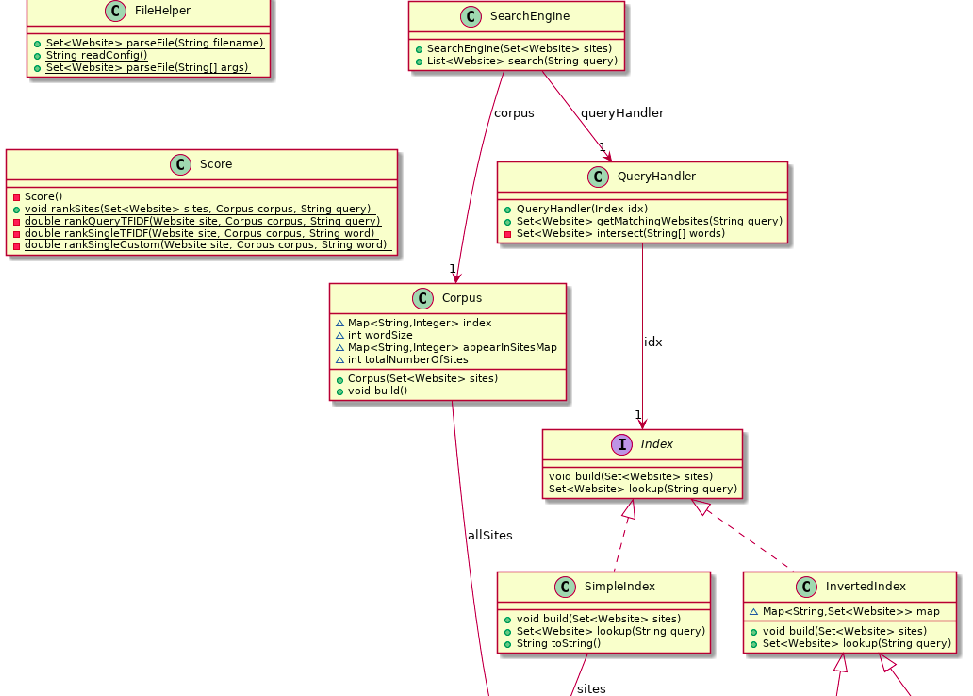
\includegraphics[width=\textwidth]{graphics/uml/ScoreAsUtilityZoom.png}
	\caption{UML Diagram for the search-engine when Score is a utility class.}
	\label{fig:uml:ScoreAsUtility}
\end{figure}

In the first implementation we tried, we wrote a utility class named \code{Score} which had static rank methods for ranking websites.   
A UML class diagram for this design is shown if figure \ref{fig:uml:utilityClass}, and snippets of relevant code lines from the implementation is shown in listing \ref{lst:ScoreUtilityClass}. 
A drawback of this method is that it doesn't have a \code{Score} interface as specified in the mandatory requirements for the assignment.  

Another drawback of this implementation is that the ranking functions work by having a sideeffect, rather than returning a value. The ranking method sets a score field in the website. This field is then used when sorting the sites. A better way would have been to make ranking functions with no sideeffect and instead return the website score directly.
This is fixed in the second implementation we did.      

\begin{lstlisting}[language=Java, caption=This is a code example., label=lst:ScoreUtilityClass]
//// From Score class 

/**
* Rank the sites according to the whole query. I.e calculate and set the rank field of each
* website in the supplied set. The ranking algorithm we have chosen is TFIDF.
* 
* @param sites a set of websites that are to be ranked.
* @param corpus the corpus of all websites.
* @param query the searh query.
* 
* @return the method has no return value. But the methods side effect is to set the rank field
*         for the supplied set of websites.
*/
public static void rankSites(Set<Website> sites, Corpus corpus, String query) {
	for (Website site : sites) {
		site.setRank(rankQueryTFIDF(site, corpus, query)); // bad decision! 
					// better just to use double from rankQueryTFIDF() and do the sorting imidiately. 
	}
}
\end{lstlisting}

\begin{lstlisting}[language=Java, caption=This is a code example., label=lst:ScoreUtilityClass-2]
//// From SearchEngine 

	Set<Website> results = queryHandler.getMatchingWebsites(query);
	
	// rank the websites that matches the query
	Score.rankSites(results, this.corpus, query); // using the static method Score.rankSites.
	
	// OBS: convert a set of websites to a list, since the sort method only works for list.
	List<Website> resultList = results.stream().collect(Collectors.toList());  
	
	// make a Comparator from the static method Comparator.comparingDouble()
	Comparator<Website> rankComparator = Comparator.comparingDouble(Website::getRank);
	resultList.sort(rankComparator.reversed()); 

//// From Website

	/**
	*  Set the rank of the site. This method is used by an external ranking method
	* to set the rank of the site. 
	* 
	* @param rank the rank that is to be assigned to the website.  
	*/
	public void setRank(double rank) {
		this.rank = rank;
	}

	/**
	* Returns the currently assigned rank of the website. 
	* 
	* @return the current rank of the website. 
	*/
	public double getRank() {
		return rank;
	}
\end{lstlisting}


\subsubsection{Option 2: Score as Interface}
\begin{figure}[t]
	\centering
	%\includegraphics[width=\textwidth]{graphics/..}
	\caption{UML Diagram for search-engine when using an interface Score.}
	\label{fig:uml:score-as-interface}
\end{figure}
Another option which largely preserves the same division of responsibility is shown in the class diagram in figure \ref{fig:uml:score-as-interface}.    
This is the solution we went with in our final version of the code (version...). Relevant coding lines from the implementation is shown in listing \ref{lst:scoreInterface}.

This solution has the \code{Score} interface as required. Another big improvement we made, was to remove the score/rank field from \code{Website}, and instead use the value from \code{rankTFIDF()} directly to do the sorting.  




\begin{lstlisting}[language={Java}, caption={This is a code example.}, label={lst:scoreInterface}]
//// From TFIDFScore class 

// Rank the site according to the whole query, and the Corpus.
@Override
public Double rank(Website site, Corpus corpus, String query) {
	return rankQueryTFIDF(site, corpus, query);
}


//// From SearchEngine 

/**
* Rank a list of websites, according to the query, 
* also using information about the whole database from corpus object. 
*
* @param list List of websites to be ordered according to rank.
* @param query The search query.
* @return return the list of websites reordered according to rank.
* I.e the method modifies the input list.  
*/
private List<Website> orderWebsites(List<Website> list, String query) {
	// create a nested Comparator class
	class RankComparator implements Comparator<Website> {
		public int compare(Website site, Website otherSite) {
			return score.rank(site, corpus, query).compareTo(score.rank(otherSite, corpus, query));
		}
	}

	// sort the websites according to their rank.
	list.sort(new RankComparator().reversed());     
	return list;
}
\end{lstlisting}



